% Based on https://tex.stackexchange.com/questions/47377/proper-nesting-of-tikzpicture-environments-reset-all-pgf-values-to-their-defaul

\providecommand{\home}{../../..}
\documentclass[\home/main.tex]{subfiles}
\usetikzlibrary[arrows,snakes,backgrounds]
\usetikzlibrary{patterns}
\usetikzlibrary{positioning,fit}
\usetikzlibrary{decorations.markings}

\begin{document}

% -------------------------------------------------
%           NEURAL NETWORK MACRO
% -------------------------------------------------

\def\layersep{1.5cm}

% import from mlp.tex
\newsavebox{\neuralnetworkBox}
\sbox{\neuralnetworkBox}{%
    \begin{tikzpicture}[
            shorten >=1pt,->,
            draw=black!50,
            node distance=\layersep,
            every pin edge/.style={<-,shorten <=1pt},
            neuron/.style={circle,fill=black!25,minimum size=17pt,inner sep=0pt},
            input neuron/.style={neuron, fill=ColorAccent1},
            output neuron/.style={neuron, fill=ColorAccent2},
            hidden neuron/.style={neuron, fill=ColorMainLight},
            annot/.style={text width=4em, text centered}
        ]
        % set number of hidden layers
        \newcommand\Ninputs{4}
        \newcommand\Nhidden{2}
        \newcommand\NhiddenNeurons{5}
        \newcommand\Noutputs{3}
        \newcommand\OffsetOutputLayer{-0.5cm}

        % Draw the input layer nodes
        \foreach \name / \y in {1,...,\Ninputs}
        % This is the same as writing \foreach \name / \y in {1/1,2/2,3/3,4/4}
        % \node[input neuron, pin=left:Input \#\y] (I-\name) at (0,-\y) {};
        \node[input neuron] (I-\name) at (0,-\y) {};

        % Draw the hidden layer nodes
        \foreach \N in {1,...,\Nhidden} {
                \foreach \y in {1,...,\NhiddenNeurons} {
                        \path[yshift=0.5cm]
                        node[hidden neuron] (H\N-\y) at (\N*\layersep,-\y cm) {};
                    }
                \node[annot,above of=H\N-1, node distance=1cm] (hl\N) {};
            }

        % Draw the output layer node
        % \node[output neuron,pin={[pin edge={->}]right:Output}, right of=H\Nhidden-3] (O) {};
        % \node[output neuron, right of=H\Nhidden-3] (O) {};
        \foreach \y in {1,...,\Noutputs} {
                \path[yshift=\OffsetOutputLayer] node[output neuron, right of=H\Nhidden-3] (OUT-\y) at (\Nhidden*\layersep,-\y cm) {};
            }


        % Connect every node in the input layer with every node in the hidden layer.
        \foreach \source in {1,...,\Ninputs}
        \foreach \dest in {1,...,\NhiddenNeurons}
        \path (I-\source) edge (H1-\dest);

        % connect all hidden stuff
        \foreach [remember=\N as \lastN (initially 1)] \N in {2,...,\Nhidden}
        \foreach \source in {1,...,\NhiddenNeurons}
        \foreach \dest in {1,...,\NhiddenNeurons}
        \path (H\lastN-\source) edge (H\N-\dest);

        % Connect every node in the hidden layer with the output layer
        \foreach \source in {1,...,\NhiddenNeurons}
        \foreach \dest in {1,...,\Noutputs}
        \path (H\Nhidden-\source) edge (OUT-\dest);

        % Annotate the layers
        % \node[annot,left of=hl1] {Inputs};
        % \node[annot,right of=hl\Nhidden] {Outputs};

    \end{tikzpicture}
}

\newcommand{\scaledMLP}[2]{\resizebox{#1}{#2}{\usebox{\neuralnetworkBox}}}
\newcommand{\scaledMLPWidth}[1]{\resizebox{#1}{!}{\usebox{\neuralnetworkBox}}}
\newcommand{\scaledMLPHeight}[1]{\resizebox{!}{#1}{\usebox{\neuralnetworkBox}}}

% -------------------------------------------------
%           ROBOT ACTION MACRO
% -------------------------------------------------
% copy from fig-robot-arm

% Define a variable as a length
\newcommand{\nvar}[2]{%
    \newlength{#1}
    \setlength{#1}{#2}
}

% Define a few constants for drawing
\nvar{\dg}{0.3cm}
\def\dw{0.25}\def\dh{0.5}
% Define commands for links, joints and such
\def\link{\draw [double distance=1.5mm, very thick] (0,0)--}
\def\joint{%
    \filldraw [fill=white] (0,0) circle (5pt);
    \fill[black] circle (2pt);
}
\def\grip{%
    \draw[ultra thick](0cm,\dg)--(0cm,-\dg);
    \fill (0cm, 0.5\dg)+(0cm,1.5pt) -- +(0.6\dg,0cm) -- +(0pt,-1.5pt);
    \fill (0cm, -0.5\dg)+(0cm,1.5pt) -- +(0.6\dg,0cm) -- +(0pt,-1.5pt);
}

\def\robotbase{%
    \draw[rounded corners=8pt] (-\dw,-\dh)-- (-\dw, 0) --
    (0,\dh)--(\dw,0)--(\dw,-\dh);
    \draw (-0.5,-\dh)-- (0.5,-\dh);
    \fill[pattern=north east lines] (-0.5,-1) rectangle (0.5,-\dh);
}

% This macro draws a three link manipulator.
% Input parameters:
%   #1 theta_1
%   #2 L_1
%   #3 theta_2
%   #4 L_2
%   #5 theta_3
%   #6 L_3
%
% Example:
%   \threelink{60}{2}{-70}{2}{30}{1}
\newcommand{\threelink}[6]{%
    \robotbase
    \link(#1:#2);
    \joint
    \begin{scope}[shift=(#1:#2), rotate=#1]
        \link(#3:#4);
        \joint
        \begin{scope}[shift=(#3:#4), rotate=#3,draw=ColorAccent2Strong]
            \link(#5:#6);
            \joint
            \begin{scope}[shift=(#5:#6), rotate=#5]
                \grip
            \end{scope}
        \end{scope}
    \end{scope}
}

\newsavebox{\robotActionBox}
\sbox{\robotActionBox}{%
    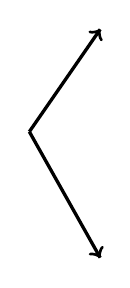
\begin{tikzpicture}
        % Need to reimport, dunno why though
        \usetikzlibrary{patterns}
        \usetikzlibrary{decorations.markings}
        \begin{scope}
            \threelink{70}{2}{-130}{2}{60}{1}
        \end{scope}

        \begin{scope}[xshift=4cm,yshift=2cm,scale=0.5, every node/.append style={transform shape}]
            \threelink{60}{2}{-110}{2}{90}{1}
        \end{scope}

        \begin{scope}[xshift=4cm,yshift=-2cm,scale=0.5, every node/.append style={transform shape}]
            \threelink{60}{2}{-110}{2}{30}{1}
        \end{scope}

        % draw arrows between the scopes above
        \begin{scope}[very thick,decoration={
                        markings,
                        mark=at position 1.0 with {\arrow{>}}}
            ]
            \draw[postaction={decorate}] (3,0.15)--(3.9,1.45);
            \draw[postaction={decorate}] (3,0.15)--(3.9,-1.45);
        \end{scope}
    \end{tikzpicture}
}

\newcommand{\scaledRobotAction}[2]{\resizebox{#1}{#2}{\usebox{\robotActionBox}}}
\newcommand{\scaledRobotActionWidth}[1]{\resizebox{#1}{!}{\usebox{\robotActionBox}}}
\newcommand{\scaledRobotActionHeight}[1]{\resizebox{!}{#1}{\usebox{\robotActionBox}}}
% ====================================================================================================
%           FINAL PICTURE
% ====================================================================================================
\begin{tikzpicture}[node distance = 10em, auto, thick]
    \tikzset{
        block/.style={
                rectangle, draw, text width=8em, text centered, rounded corners,
                minimum height=4em,minimum width=10em
            },
        descr/.style={
                fill=white,
                inner sep=2.5pt
            },
        connector/.style={
                -latex,
                font=\scriptsize
            },
        % Based on https://tex.stackexchange.com/questions/50780/arrows-at-right-angles-on-a-tikzpicture-matrix
        rectangle connector/.style={
                connector,
                to path={(\tikztostart) -- ++(#1,0pt) |- (\tikztotarget)  \tikztonodes },
                pos=0.25
            },
        rectangle connector/.default=-2cm,
        straight connector/.style={
                connector,
                to path=--(\tikztotarget) \tikztonodes
            }
    }

    \node[block]        (agent)     [align=center]                      {Agent\\\scaledMLPHeight{2cm}};
    \node[block]        (env)       [below of=agent]                    {Environment};
    \node[]             (envPicture)[below of=env, node distance=6em]                      {\includegraphics[width=.30\textwidth]{\home/chapters/02-sota/figures/baxter_in_env_50p.jpg}};

    % Don't delete this, this is how I did it manually without \tikztonodes macro magic 
    % \draw [->] (env) to node [auto, swap] {Reward} (agent);
    % \draw [->] (env.west) -- ++(-0.5,0) |- node[pos=0.25] {State} (agent.west); % first go left a bit, then go vertical and horizontal to agent node while putting a label with name "State" on it
    % \draw [->] (agent.east) --++(0.5,0) |- node[pos=0.25] {Action}               (env.east);

    \draw [straight connector] (env) to node [descr, swap] {Reward $r_{t+1}$} (agent);
    \draw [rectangle connector=0.5cm] (agent.east) to node[descr,align=left, pos=0,xshift=0.5cm,yshift=-2cm] {\textcolor{ColorAccent2Strong}{Action $a_{t}$}\\\scaledRobotActionHeight{2cm} } (env.east);
    \draw [rectangle connector=-0.5cm] (env.west) to node[descr,align=center, pos=1,xshift=-2.5cm,yshift=-3.0cm] {\textcolor{ColorAccent1Strong}{State $s_{t}$}\\\includegraphics[width=2.5cm, height=2.0cm]{\home/chapters/02-sota/figures/baxter_state_example_annotated.jpg}} (agent.west);


\end{tikzpicture}
\end{document}
